\section{Implementation, Integration and Test Plan}
The whole system is divided in two parts: the forum and the data aggregator. Both presents the same components that are:
\begin{itemize}
    \item Client: the website which is load by the web browser.
    \item Web Server (that also include the Service Provider Module).
    \item Application Server.
    \item Internal Database.
    \item External services such as IdP and the public datasources.
\end{itemize}
These elements will be implemented following a bottom up approach, in order to have an easy implementation and testing.
The main focus will be on the Application Server module because is the most complex part considering it is the core of the application and it also requires more testing.\\
The following table presents the main functionalities of the system, highlighting for each of them the importance for the costumer and the difficulty of its implementation. 

\begin{table}[h!]
    \caption{Implementention and testing precedences}
    \label{tab:implementention_testing_precedences}
    \rowcolors{2}{gray!25}{white}
    \centering
    \begin{tabular}{c|c|c|c}
    \rowcolor{gray!50}
    \textbf{Functionality} & \textbf{Module} & \textbf{Importance for customer} & \textbf{Difficulty}\\ \hline\hline
    Sign up and Login & 6 & High & Low\\
    Forum & 3 & High & High\\
    Notification & 1 & Low & Low\\
    Downloader & 1 & Medium & High\\
    Deviance & 1 & High & High\\
    Data aggregator & 1 & High & High\\\hline
    \end{tabular}
\end{table}

All the modules described in this document relies on a DBMS for each sub-system (one for the forum and another one for the data aggregator) that has to be implemented firstly.\\
According to table \ref{tab:implementention_testing_precedences} we decide to implement the functionalities following their importance.

\begin{itemize}
    \item \textbf{Sign up and Login:} the two functionalities are available in both subsystems and they are strictly related because of the adoption on the Identity Provider; in fact, a SignUp is the result of the first login. For that reason is a good choice to first implement the login function that also implies to set up the Shibboleth Service Provider Module and connect it to a test IdP and then implement the sign up method.
    The adoption of a the Service Provider module ensure that User attributes are available in the server session so a custom endpoint is needed to read and save them in the DBMS for further uses.\\
    In this parts is is also important to test the ability to save and retrieve User attributes from the DBMS correctly. 
    
    \item \textbf{Forum:} This functionality represents the core of the forum. It is implemented by means of the TopicManager, DiscussionManager and the PostManager which merged provides all the functionalities inherent to discussions; but also is implemented by means of the UserManager. In this part the DBMS cover a fundamental role because all the managed data have to be saved.\\
    The testing is done using automated test class. In fact a valid User and a valid Policy maker accounts are required, a discussion has to be created and some post added, modified and deleted by multiple and different controllers calls.
    
    \item \textbf{Data aggregator:} This functionality represents the core of the homonym sub-system. It is implemented by means of the DataManager and the AdministratorManager which provide the method needed to add, delete and modify data sources (by the Administrator) and methods to save, get and filter data from the DBMS.
    The testing is done using an automated test class for the same reason of the Forum described above.
    
    \item \textbf{Deviance:} This functionality is strictly related to a Policy maker activity in the Data aggregator sub-system. It consist in the ability of using one or multiple data sets to calculate a ranking of a specific area using predefined parameters or custom ones. This is implemented by means of the DataManager (get, store data in the DBMS and also manage the specific algorithm calculation and the parameter management) and the UserManager which is used to get the Area in which the Policy maker works. The testing could be done by an automated test class but also a hand check is required to verify if the resulting ranking is coherent with the expected estimation in some more general cases. 
    
    \item \textbf{Downloader:} It represents the principal service of the data aggregator sub-system which is responsible to connect to external data sources, fetch them and save the received content periodically.
    This function requires also some entities described in the Data aggregator to identity and parse the content correctly. Also the functionalities of saving data in the DBMS are provided by the Data aggregator.
    
    \item \textbf{Notification:} This functionality is implemented through the NotificationManager. To test the system will be necessary to use the Forum functionality and verify that the system works either if a Policy maker approve the publication or if he decides to decline it. Different User will be needed to see if the notification functionality works also for the one who follows the discussion.
\end{itemize}

\subsection{Clarification on component integration}
In this section is present an overall description about how the components are integrated and how they communicate between each other.\\

\subsubsection{Components Integration Forum}
\begin{figure}[h!]
        \centering
        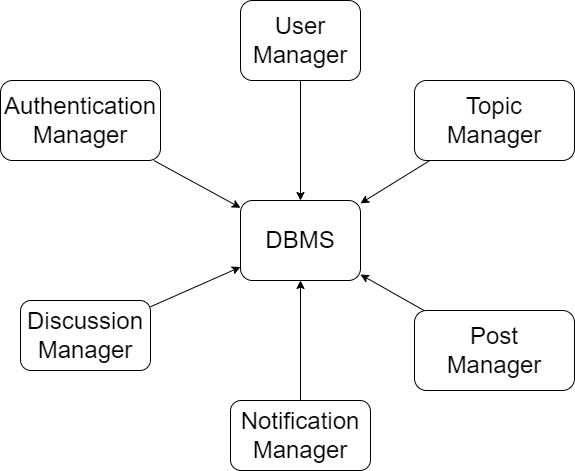
\includegraphics[scale=0.5]{images/component_integration/components_integration_forum.png}
        \caption{Components Integration Forum}
        \label{fig:components_integration_forum}
\end{figure}
\FloatBarrier

\newpage
\subsubsection{Components Integration Data}
\begin{figure}[h!]
        \centering
        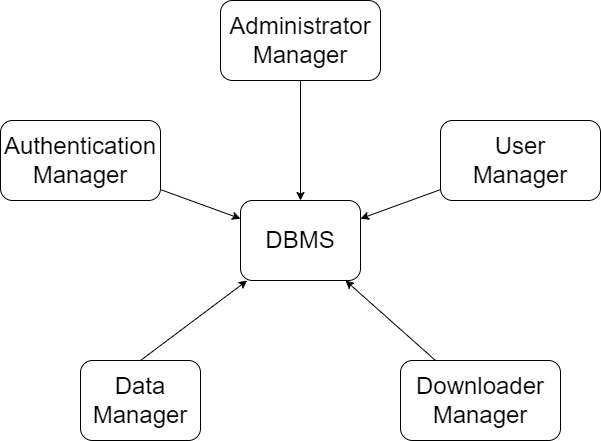
\includegraphics[scale=0.5]{images/component_integration/components_integration_data.png}
        \caption{Components Integration Data}
        \label{fig:components_integration_data}
\end{figure}
\FloatBarrier

Using the bottom up method of implementation, for both the Forum and the Data sub-system, the first component to create is the DBMS. To go on, the main application component will have to be integrated with it.

\subsubsection{IdP Integration}
\begin{figure}[h!]
        \centering
        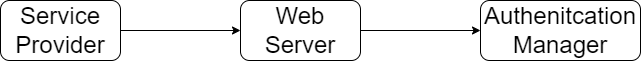
\includegraphics[scale=0.5]{images/component_integration/idp_integration.png}
        \caption{IdP Integration}
        \label{fig:idp_integration}
\end{figure}
\FloatBarrier

The ability to use external Identity Provider requires an integration between the ServiceProviderModule with the AuthenticationManager by means of the WebServerModule. In fact a ServiceProvider (like Shibboleth) acts as a plugin for the web server to protect a resource. In our case the "..dream/login" path represents the resource to be protected that is the endpoint of the AuthenticationManager to complete the login flow.

\newpage
\subsubsection{ClientManager Integration Forum}
\begin{figure}[h!]
        \centering
        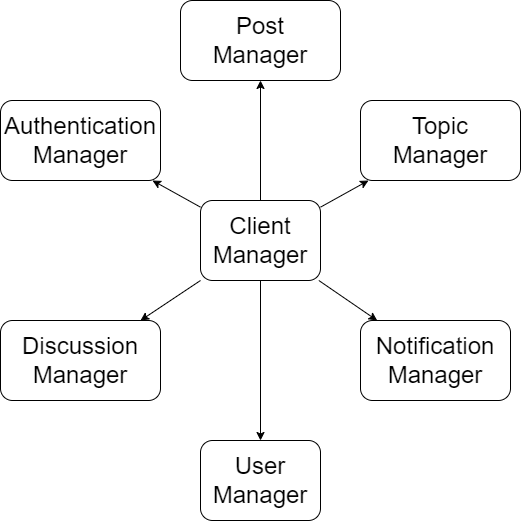
\includegraphics[scale=0.5]{images/component_integration/client_manager_forum_integration.png}
        \caption{ClientManager Integration Forum}
        \label{fig:client_manager_integration_forum}
\end{figure}
\FloatBarrier

\newpage
\subsubsection{ClientManager Integration Data}
\begin{figure}[h!]
        \centering
        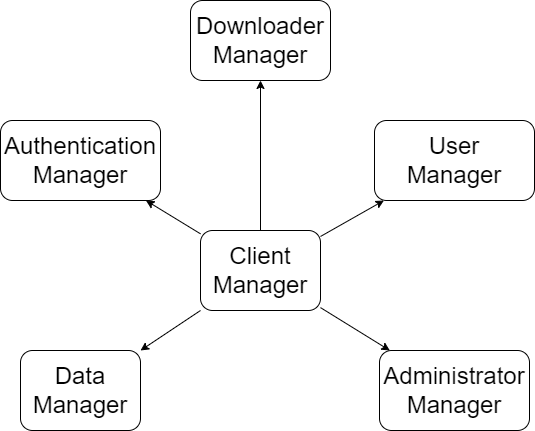
\includegraphics[scale=0.5]{images/component_integration/client_manager_data_integration.png}
        \caption{ClientManager Integration Data}
        \label{fig:client_manager_integration_data}
\end{figure}
\FloatBarrier

Then, will be integrated the ClientManager, for both the Forum and the Data sub-system, as shown correspondingly in figure \ref{fig:client_manager_integration_forum} and in figure \ref{fig:client_manager_integration_data}. Integrating those, will let the user to exploit all the functionalities they are allowed to.

\subsubsection{Client-Server Integration}
\begin{figure}[h!]
        \centering
        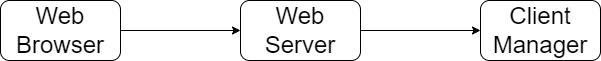
\includegraphics[scale=0.5]{images/component_integration/client_server_integration.png}
        \caption{Client-Server Integration}
        \label{fig:client_server_integration}
\end{figure}
\FloatBarrier

Finally, it is possible to integrate the web server module and the web browser module, as shown in figure \ref{fig:client_server_integration}. This part brings the integration of the client-server communication.